%%%%%%%%%%%%%%%%%%%%%%%%%%%%%%% SGD 
\begin{frame}{Optimisation Program}
  Let $\dataset = (\exi,\class\sid{i})_{i=1}^n = (\datax,\datac)$, and a  logistic regression model, $\params =  (w_0, \vct{w})$. \\
  \begin{block}{The loss function}
  $$
  \fullloss = - log(P(\datac | \datax, \params) ) = -
  \big(\sum_{i=1}^n \class\sid{i} log(\bern\sid{i} )+ (1-\class\sid{i}) log(1-\bern\sid{i} )
  \big)
  $$
  
  with:
  $$       \bern\sid{i} = \sigma(w_0 + \scal{\vct{w}}{\exi})  = \frac{1}{1+e^{-(w_0 + \scal{\vct{w}}{\exi})}}$$
\end{block}



\begin{block}{Learning = optimisation}
  \begin{center}
    Find $\params$ in ordre to minimize $\fullloss$ ?
  \end{center}
\end{block}
\end{frame}


\begin{frame}{Function minimization}
  \begin{block}{Bad news}
    No closed form solution in general ! 
  \end{block}
  \begin{block}{Good news}
    \begin{itemize}
    \item The function is convex \textit{w.r.t} $\params$
    \item Convex functions are ``easy'' to minimize
    \item[$\rightarrow$] An efficient, easy and generic algorirthm exists: 
      \begin{center}
        The (stochastic)  gradient descent with many variants  
      \end{center}
    \end{itemize}
  \end{block}
\end{frame}


\begin{frame}{A convex function}
  \begin{center}
    
% \shorthandoff{;} with babel french
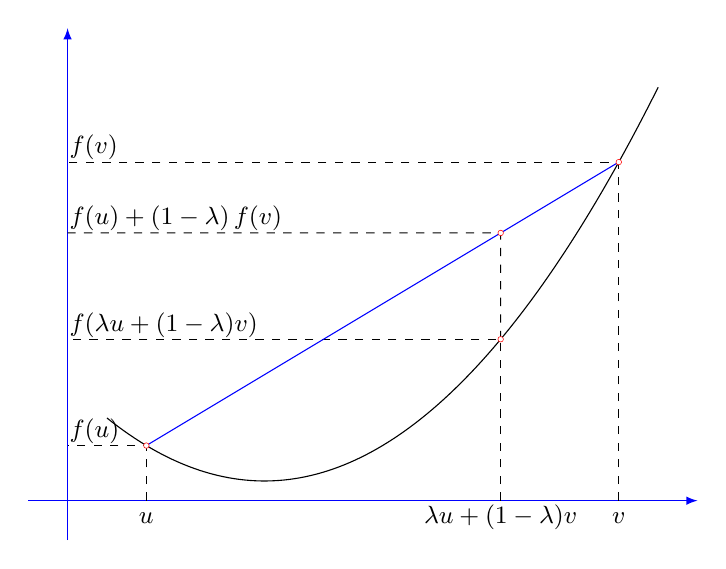
\begin{tikzpicture}[declare function={f(\x)=(\x-1)*(\x-1)/2 + 0.1;},x={(2.5cm,0)},y={(0,2.5cm)},samples=101,font=\small,inner sep=0.5pt]
  \draw[blue,-latex] (-0.2,0) -- (3.2,0);
  \draw[blue,-latex] (0,-0.2) -- (0,2.4);
  \coordinate (O) at (0,0);
  \draw plot[domain=0.2:3,variable=\x] ({\x},{f(\x)});
  \foreach [count=\Z] \X/\Y in {0.4/{u},2.2/{\lambda u +(1-\lambda) v},2.8/{v}}
  {\draw[dashed] (\X,0) coordinate (X\Z) node[below]{$\strut\Y$} -- (\X,{f(\X)}) coordinate (F\Z)
    -- (0,{f(\X)}) node[above right]{$f(\Y)$};}
  \draw[blue] (F1) -- (F3);
  \draw[dashed] (F2) --
  (intersection cs:first line={(X2)--(F2)}, second line={(F1)--(F3)})
  coordinate (F4) -- (O|-F4) node[above right]{$f(u)+(1-\lambda)\,f(v)$};
  \foreach \X in {1,...,4}
  {\draw[very thin,red,fill=white] (F\X) circle(1pt);}
\end{tikzpicture}
  
  \end{center}
$$  f\left(\lambda u +(1-\lambda)v\right)\leq \lambda\,f(u)+(1-\lambda)\,f(v).$$
\end{frame}


\begin{frame}
  \frametitle{Gradient Descent - intuition}
  How to reach the minimum ? How to recognize it ?

  % $\rightarrow$ Fonction convexe : ouf !
  %Analogie brouillard
  \begin{alertblock}{Caution :}
    \begin{itemize}
    \item The whole landscape is unknown
    \item Only pointwise knowledge: the function value and its
      (partial) derivatives
    \end{itemize}
  \end{alertblock}
  \begin{center}
    \includegraphics[width=0.5\textwidth]{./figs/brouillard.jpg}
  \end{center} 
\end{frame}


\begin{frame}{Interpretation of partial derivative}
  \begin{columns}
    \begin{column}{0.5\textwidth}
      \includegraphics[width=0.9\textwidth]{./figs/derive_1.pdf}
    \end{column}
    \begin{column}{0.5\textwidth}
      \begin{align*}
        w_k &= w_k + \eta \frac{\partial \ploss(\params,\exi,\classi) }{\partial
          w_k}\ \\
        &\ploss(\params,\exi,\classi) \nearrow
      \end{align*}
    \end{column}
  \end{columns}
  \begin{columns}
    \begin{column}{0.5\textwidth}
      \includegraphics[width=0.9\textwidth]{./figs/derive_2.pdf}
    \end{column}
    \begin{column}{0.5\textwidth}
      \begin{align*}
        w_k &= w_k - \eta \frac{\partial \ploss(\params,\exi,\classi)}{\partial
          w_k}\ \\
         &\ploss(\params,\exi,\classi) \searrow
      \end{align*}
\end{column}
  \end{columns}
  \begin{center}
\important{    $\eta > 0$ and small}
  \end{center}
\end{frame}


\begin{frame}{Minimization of  $\ploss$ \textit{w.r.t} $w_k$}

  \begin{columns}[c]
    
    \column{.5\textwidth}
    \begin{block}{Sketch}
      \setbeamertemplate{enumerate items}[default]
      \begin{enumerate} \setcounter{enumi}{-1}
      \item Start from a random point, 
      \item evaluate the slope, 
      \item follow it a bit, and \\loop back to the previous step
    \end{enumerate}
    \end{block}
    
    \column{.4\textwidth}
    \begin{center}
      \includegraphics[width=\textwidth]{./figs/velo.jpg}
    \end{center}
    
  \end{columns}

  \begin{block}{Algorithm}
    \begin{itemize}
    \item Pick $\eta>0$ and the initial value of $w_k$.
    \item while \textit{true} :
      \begin{itemize}
      \item compute $\ploss(\params,\exi,\classi)$

      \item compute the derivative and update $w_k$
$$      w_k= w_k - \eta \frac{\partial \ploss(\params,\exi,\classi) }{\partial
  w_k}
$$
\end{itemize}
\end{itemize}
\end{block}
\end{frame}

\begin{frame}{``Convergence'' }
At the minimum: 
  $$
\frac{\partial \ploss(\params,\exi,\classi) }{\partial
  w_k}  = 0
$$
\begin{center}
  \includegraphics[width=0.6\textwidth]{./figs/derive_null.pdf}
\end{center}

\end{frame}


\begin{frame}
  \frametitle{The learning rate : $\eta$}

\begin{itemize}
  \item small  steps: a valid approximation but boring ! 
  \item large steps: oscillation and divergence 
\end{itemize}
  \begin{center}
    \includegraphics[width=\textwidth]{./figs/pas.jpg}
  \end{center}

  \begin{itemize}
    \item Constant or adaptative $\eta$
    \item This is the role of the \textit{optimizer} !
  \end{itemize}
\end{frame}


\begin{frame}{Generalization : the gradient}
  \begin{itemize}
  \item All the parameters are in one vector : $\params = (w_0,\vct{w}) = (w_0,w_1,w_2,... ,w_{\nfeats})$
  \item Compute all the partial derivatives and store them in one
    vector: 
    \begin{displaymath}
              \left(
          \begin{array}{l}
            \partial{\ploss(\params,\exi,\classi)}/\partial{w_0}\\
            \partial{\ploss(\params,\exi,\classi)}/\partial{w_1}\\
            \partial{\ploss(\params,\exi,\classi)}/\partial{w_2}\\
...\\
            \partial{\ploss(\params,\exi,\classi)}/\partial{w_{\nfeats}}
            \end{array} 
          \right) = \vgrad{\params,\exi,\classi}{\ploss}
    \end{displaymath}
  \end{itemize}
  
  \begin{center}
    $\vgrad{\params}{\ploss}$ is the gradient (vector)  of $l$ w.r.t $\params$.
  \end{center}
\end{frame}

\begin{frame}{Gradient descent in 2D }
  \begin{center}
    \includegraphics[width=0.6\textwidth]{./figs/sgd}
  \end{center}
\end{frame}


\begin{frame}{Gradient descent: the algorithm}
  \framesubtitle{Batch / Online}
  \begin{block}{Batch minimization}
    while: 
        \begin{displaymath}
          \left.
            \begin{array}{ll}
              \textrm{Pour } i = 1 ... n : \\
              &\fullloss +=   \ploss(\params,\exi,\classi) \\
              &\vgrad{\params}{\fullloss} += \vgrad{\params}{  \ploss(\params,\exi,\classi)  } \\
              \params = \params - \eta  \vgrad{\params}{\fullloss}
            \end{array}\right\} \textrm{ one epoch}
        \end{displaymath}
  \end{block}

  \begin{block}{Stochastic Gradient Descent}
    while: 
        \begin{displaymath}
          \left.
            \begin{array}{ll}
              \textrm{shuffle } \dataset\\
              \textrm{for } i = 1 ... n : \\
              &\fullloss +=   \ploss(\params,\exi,\classi) \\
              &\params = \params - \eta \vgrad{\params}{\ploss(\params,\exi,\classi)  } \\
            \end{array}\right\} \textrm{ one epoch}
        \end{displaymath}
  \end{block}
  \begin{center}
    \important{A trade-off: the mini-batch}
  \end{center}
  \end{frame}

  \begin{frame}{A terminololy point}
    \begin{block}{Gradient Descent}
      A simple yet efficient algorithm to minimize a convex function
    \end{block}
    \begin{block}{Batch \textit{vs} Online}
      \begin{itemize}
      \item Batch: consider the whole $\dataset$ to estimate the gradient and the update
      \item Online: consider the training examples one by one
      \item Mini-batch: the trade-off
      \end{itemize}
    \end{block}
    \begin{block}{Stochastic}
      For online and mini-batch training: randomize the order in $\dataset$
    \end{block}
  \end{frame}